
\documentclass[10pt,a4paper]{report}
%\usepackage[latin1]{inputenc}
\usepackage[utf8]{inputenc}
\usepackage{amsmath}
\usepackage{amsfonts}
\usepackage{amssymb}
\usepackage{graphicx}
\usepackage{multicol}
\usepackage{tabularx}
\usepackage{mathtools}
\usepackage{tikz}
\usetikzlibrary{arrows,shapes,automata,petri,positioning,calc}
\usepackage{hyperref}
\usepackage{tikz}
\usetikzlibrary{matrix,calc}
\usepackage[margin=0.5in]{geometry}
% ---- power functions -----% 
\newcommand{\myvec}[1]{\ensuremath{\begin{pmatrix}#1\end{pmatrix}}}
\let\vec\mathbf

\providecommand{\norm}[1]{\left\lVert#1\right\rVert}
\providecommand{\abs}[1]{\left\vert#1\right\vert}
\let\vec\mathbf

\newcommand{\mydet}[1]{\ensuremath{\begin{vmatrix}#1\end{vmatrix}}}
\providecommand{\brak}[1]{\ensuremath{\left(#1\right)}}
\providecommand{\lbrak}[1]{\ensuremath{\left(#1\right.}}
\providecommand{\rbrak}[1]{\ensuremath{\left.#1\right)}}
\providecommand{\sbrak}[1]{\ensuremath{{}\left[#1\right]}}
%-------end power functions----%
\newenvironment{Figure}
  {\par\medskip\noindent\minipage{\linewidth}}
  {\endminipage\par\medskip}
\begin{document}
%--------------------logo figure-------------------------%
\begin{figure*}[!tbp]
  \centering
  \begin{minipage}[b]{0.4\textwidth}

\includegraphics[scale=0.05]{../../../Downloads/iitlogo.jpg} 
  \end{minipage}
  \hfill
  \vspace{5mm}\begin{minipage}[b]{0.4\textwidth}
\raggedleft  
\includegraphics[scale=0.10]{../../../Downloads/nrc.jpeg} 

  \end{minipage}\vspace{0.2cm}
\end{figure*}
%--------------------name & rollno-----------------------
\raggedright \textbf{Name}:\hspace{1mm} YADATI KRISHNA\hspace{3cm} \Large \textbf{Assignment-5}\hspace{2.5cm} % 
\normalsize \textbf{Roll No.} :\hspace{1mm} FWC22036\vspace{1cm}
\begin{multicols}{2}

%----------------problem statement--------------%
\raggedright \textbf{Problem Statement:}\vspace{2mm}
\raggedright \\Find the equations of circle passing through (-4,3) and touching the lines x+y=2 and x-y=2 .\\
\vspace{5mm}

%-----------------------------solution---------------------------
\raggedright \textbf{SOLUTION}:\vspace{2mm}\\

%---------given----------------%
\raggedright \textbf{Given}:\vspace{2mm}\\
Equation of lines\\ 
\begin{align}
    \label{eq:line_norm_eq}
	\vec{n_1}^{\top}\vec{x} =\vec{c_1} 
\end{align}\\  
\begin{align}
    \label{eq:line_norm_eq1}
	\vec{n_2}^{\top}\vec{x} =\vec{c_2} 
\end{align}\\  
 \vspace{1mm}
Point on the circle\begin{align}
\vec{P}=\myvec{-4\\
3}
\end{align}


%-------------To find ------------------%
\textbf{To Find }\vspace{2mm}\\
Equations of circle  passing through $\vec{P}$ and touching the lines \vspace{5mm}  \\ 
%--------------steps----------------------%
\textbf{STEP-1}\vspace{2mm}\\
 \begin{align}
			    x  +y &= 2
			    \\
			    x -y  &= 2
			    \\
			    \implies 
			    \myvec{1 &  1
			    \\
			    1 & -1}\vec{x} &= \myvec{2 \\ 2}
		    \end{align}
		    
		    The augmented matrix for the above matrix equation is 
		   
		   \begin{align}
			    \myvec{
				    1 & 1 & \vrule & 2
			    \\
			    1 & -1  &\vrule & 2
		    }
		    \\
		    \xleftrightarrow[]{R_2 \leftarrow R_2 -R_1 }
			    \myvec{
				    1 & 1 & \vrule & 2
			    \\
			    0 & -2  &\vrule & 0
		    }
		    \\
		    \xleftrightarrow[]{R_2 \leftarrow R_2 /(-2) }
			    \myvec{
				    1 & 1 & \vrule & 2
			    \\
			    0 & 1  &\vrule & 0
		    }
		      \\
		    \xleftrightarrow[]{R_1 \leftarrow R_1 -R_2 }
			    \myvec{
				    1 & 0 & \vrule & 2
			    \\
			    0 & 1  &\vrule & 0
		    }
			    \implies \vec{x} = \myvec{2 \\ 0}
		    \end{align}
 \textbf{STEP-2}\vspace{2mm}\\
Let $\vec{O}$ be the centre of the circle.\\
 \vspace{2mm}
Angle of Bi-sectors for the given line equations are:\\
\begin{align}
\vec{m_1}=\myvec{1\\
-1}
\end{align} 
\begin{align}
\vec{m_2}=\myvec{-1\\
-1}
\end{align} \\
\begin{align}
\vec{m_1}-\vec{m_2}=\myvec{2\\
0}
\end{align} \\
The equation of line passing through $\vec{x}$ with normal vector $\vec{n}$ is given by\\
\begin{align}
  \label{eq:line_norm_eq2}
\vec{n}^{\top} (\vec{X-x})=0
\end{align}\\
where 
\begin{align}
  \label{eq:line_norm_eq3}
\vec{n}=\myvec{0\\
-2}
\end{align} \\
\begin{align}
  \label{eq:line_norm_eq4}
(\vec{X}-\vec{x})=\myvec{x-2\\
y-0}
\end{align} \\
on substituting \eqref{eq:line_norm_eq4}, \eqref{eq:line_norm_eq3} in \eqref{eq:line_norm_eq2} we get\\
\begin{center}
y=0
\end{center}
which means the direction vector on X-axis and hence the centre of the circle will also lie on X-axis\\
\vspace{5mm}



 Let d be the distance from centre $\vec{O}$ to line \eqref{eq:line_norm_eq}\\
 \begin{align}
  \label{conics/30/lemma}
%	\label{eq:line_dist_2d}
	d = \frac{\abs{   \vec{n}^{\top}\vec{O}-c }}{\norm{\vec{n}}}	
\end{align}
where d=r\\
So, \begin{align}
  \label{conics/30/lemma}
%	\label{eq:line_dist_2d}
	r = \frac{\abs{   \vec{n}^{\top}\vec{O}-c }}{\norm{\vec{n}}}	
\end{align}\\
Where $\vec{n}$ is normal vector of line \eqref{eq:line_norm_eq} given by\\
\begin{align}
\vec{n}=\myvec{1 \\
1} and \hspace{2mm} c=2
\end{align}\\
Substituting $\vec{n}$ , c and $\vec{O}$ in \eqref{conics/30/lemma} \\
\vspace{5mm}
Distance from $\vec{P}$ to the centre $\vec{O}$ is given by\\
\begin{align}
d = 	\norm{\vec{P}-\vec{O}}
	\label{eq:dir_line_normal_dist_pa_d}
\end{align}\\where d=r\\
Squaring on both sides\\
\begin{align}
\label{eq:dir_line_normal_dist_pa_d1}
r^2 = 	\norm{\vec{P}-\vec{O}}^2
\end{align}\\
substituting $\vec{O}$ and $\vec{P}$ in \eqref{eq:dir_line_normal_dist_pa_d1} \\

 
compare \eqref{conics/30/lemma} and\eqref{eq:dir_line_normal_dist_pa_d1} we get\\
\begin{align}
\vec{O}=\myvec{-2.65\\
0} and\hspace{2mm} \vec{O_1}=\myvec{-17.35\\
0}
\end{align}\\
From \eqref{conics/30/lemma} we get the radius as:\\
\begin{center}
r = 3.78 ,10.66
\end{center}
\vspace{1mm}
The required equations of the circles are:\\
\begin{align}
    \label{eq:conic_quad_form1}
    \vec{x}^{\top}\vec{V}\vec{x}+2\vec{u_1}^{\top}\vec{x}+f_1=0\\
     \vec{x}^{\top}\vec{V}\vec{x}+2\vec{u_2}^{\top}\vec{x}+f_2=0
    \end{align}\\
    where\\
    \begin{align}
	\label{eq:V_matrix}
	\vec{V} &= \myvec{1 & 0\\0 & 1},
	\\
	\label{eq:u_vector}
	\vec{u_1} &= \myvec{-2.65\\0}\\
	\vec{u_2} &= \myvec{-17.35\\0}
	\\
	\label{eq:fvalue}
	f_1 &= -7.26 \hspace{2mm}, f_2=187.38
	%\\
\end{align}
\begin{center}
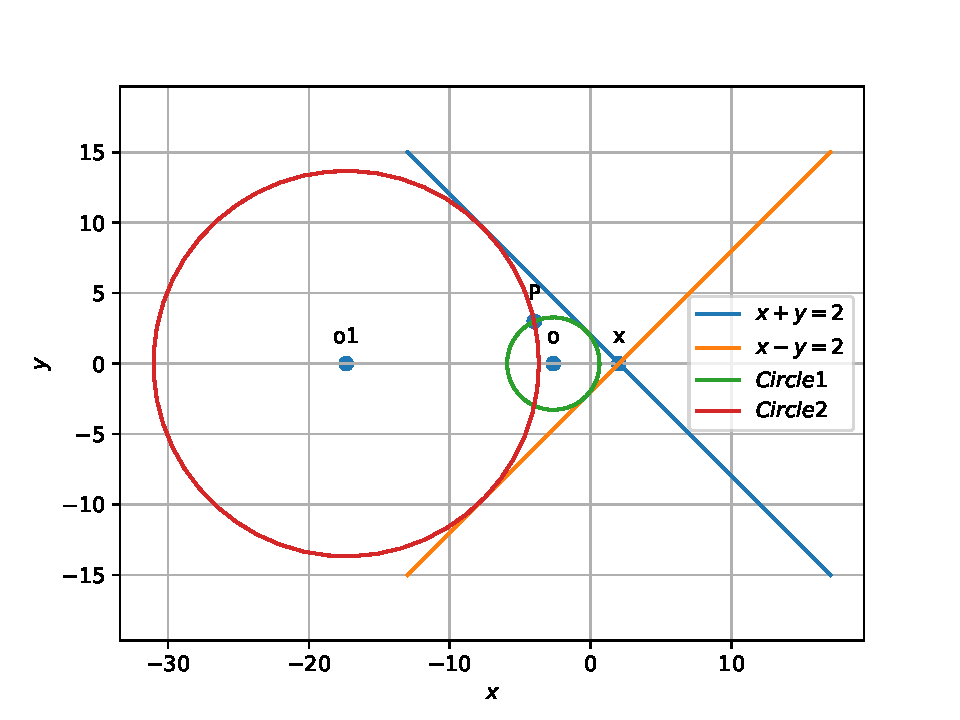
\includegraphics[scale=0.6]{../../python/figs/Circle.pdf}   
 \end{center}\vspace{1mm}
 
 \vspace{2mm} \textbf{Construction}
\begin{center}
\setlength{\arrayrulewidth}{0.5mm}
\setlength{\tabcolsep}{6pt}
\renewcommand{\arraystretch}{1.5}
    \begin{tabular}{|l|c|}
    \hline 
    \textbf{vertex} & \textbf{coordinates} \\ \hline
   $\vec{P}$ & $\myvec{
   -4\\
   3
   } $ \\\hline
      \end{tabular}
  \end{center}
  
\raggedright  Download the code \\
Github link: \href{https://github.com/KrishnaYadati/Assignments/blob/main/Matrix-line_assignment/line_program/circle.py}{Assignment-5}.
  \end{multicols}
\end{document}
